\documentclass[12pt,a4paper]{article}

% --- Page Layout -------------------------------------------------------------
\usepackage[a4paper, margin=0.8in, headheight=14pt]{geometry}

% --- Fonts (XeLaTeX) ---------------------------------------------------------
\usepackage{fontspec}
\usepackage{unicode-math}
\setmainfont{TeX Gyre Pagella}
\setmonofont[Scale=0.88]{TeX Gyre Cursor}
\setmathfont{Latin Modern Math}

% --- Packages ---------------------------------------------------------------
\usepackage{xcolor}
\usepackage{titlesec}
\usepackage{enumitem}
\usepackage{tabularx}
\usepackage{booktabs}
\usepackage{array}
\usepackage{amsmath}
\usepackage{tikz}
\usetikzlibrary{shapes.geometric, arrows.meta, positioning, calc, fit, decorations.pathreplacing}
\usepackage{tcolorbox}
\tcbuselibrary{skins, breakable}
\usepackage{hyperref}
\usepackage{fancyhdr}
\usepackage{graphicx}
\usepackage{microtype}
\hyphenpenalty=10000
\exhyphenpenalty=10000
\sloppy
\usepackage{caption}
\usepackage{setspace}
\usepackage{multirow}
\usepackage{tocloft}

% --- Q&A helper --------------------------------------------------------------
\newcommand{\Q}[1]{\textbf{#1}\par\noindent\ignorespaces}

% --- Colour Palette ----------------------------------------------------------
\definecolor{myred}{RGB}{196,30,58}
\definecolor{mydark}{RGB}{30,30,50}
\definecolor{mygreen}{RGB}{14,120,80}
\definecolor{myteal}{RGB}{0,130,140}
\definecolor{myamber}{RGB}{180,100,0}
\definecolor{mypurple}{RGB}{100,30,160}
\definecolor{mygray}{RGB}{246,247,249}
\definecolor{mgframe}{RGB}{180,185,200}
\definecolor{watermark}{RGB}{145,150,170}
\definecolor{hdrred}{RGB}{250,232,235}
\definecolor{hdrgreen}{RGB}{220,244,233}
\definecolor{hdrteal}{RGB}{220,242,244}
\definecolor{hdramber}{RGB}{253,242,215}
\definecolor{hdrpurple}{RGB}{238,228,255}
\definecolor{hdrgray}{RGB}{238,240,245}
\definecolor{rowalt}{RGB}{250,251,253}

% --- Section Formatting ------------------------------------------------------
\titleformat{\section}
  {\large\bfseries\color{myred}}{\thesection.}{0.5em}{}
  [\vspace{1pt}{\color{myred}\rule{\linewidth}{0.8pt}}]
\titleformat{\subsection}
  {\normalsize\bfseries\color{myteal}}{\thesubsection}{0.5em}{}
\titlespacing*{\section}{0pt}{18pt}{7pt}
\titlespacing*{\subsection}{0pt}{11pt}{4pt}

% --- Paragraph ---------------------------------------------------------------
\setlength{\parindent}{0pt}
\setlength{\parskip}{4pt}

% --- TOC Styling -------------------------------------------------------------
\renewcommand{\cfttoctitlefont}{\large\bfseries\color{myred}}
\renewcommand{\cftaftertoctitle}{\par\noindent{\color{myred}\rule{\linewidth}{0.8pt}}}
\setlength{\cftbeforetoctitleskip}{0pt}
\setlength{\cftaftertoctitleskip}{6pt}
\renewcommand{\cftsecfont}{\normalsize\bfseries\color{mydark}}
\renewcommand{\cftsecpagefont}{\normalsize\bfseries\color{mydark}}
\renewcommand{\cftsecleader}{\cftdotfill{\cftdotsep}}
\setlength{\cftbeforesecskip}{7pt}
\renewcommand{\cftsubsecfont}{\small\color{mydark}}
\renewcommand{\cftsubsecpagefont}{\small\color{mydark}}
\setlength{\cftbeforesubsecskip}{3pt}
\setlength{\cftsubsecindent}{1.4em}

% --- Table helpers -----------------------------------------------------------
\renewcommand{\arraystretch}{1.45}
\setlength{\tabcolsep}{6pt}
\newcolumntype{B}[1]{>{\small\bfseries\raggedright\arraybackslash}m{#1}}
\newcolumntype{Y}{>{\small\raggedright\arraybackslash}X}
\renewcommand{\tabularxcolumn}[1]{m{#1}}

% --- Header / Footer ---------------------------------------------------------
\pagestyle{fancy}
\fancyhf{}
\fancyhead[L]{\small\color{myred}\textbf{BS-CH101}\;\color{mydark}--- Chemistry-I}
\fancyhead[R]{\small\color{myteal}\textbf{Module 1 Notes}}
\fancyfoot[C]{\small\color{mydark}\thepage}
\fancyfoot[R]{\small\color{watermark}\textit{\copyright\ Biraj}}
\renewcommand{\headrulewidth}{0.5pt}
\renewcommand{\footrulewidth}{0.3pt}

% --- Hyperref ---------------------------------------------------------------
\hypersetup{
  colorlinks=true, linkcolor=myteal, urlcolor=myteal,
  pdfauthor={Biraj Sarkar},
  pdftitle={BS-CH101 --- Module 1 Notes}
}

% --- tcolorbox styles --------------------------------------------------------
\tcbset{
  tikzbox/.style={
    colback=mygray, colframe=mgframe, boxrule=0.6pt, arc=4pt,
    left=8pt, right=8pt, top=6pt, bottom=6pt,
    colbacktitle=mgframe, coltitle=mydark,
    fonttitle=\small\bfseries
  },
  defbox/.style={
    colback=hdrgreen, colframe=mygreen, boxrule=0.8pt, arc=4pt,
    left=9pt, right=9pt, top=6pt, bottom=6pt,
    colbacktitle=mygreen, coltitle=white,
    fonttitle=\small\bfseries
  },
  formulabox/.style={
    colback=hdrteal, colframe=myteal, boxrule=0.8pt, arc=4pt,
    left=9pt, right=9pt, top=7pt, bottom=7pt,
    colbacktitle=myteal, coltitle=white,
    fonttitle=\small\bfseries
  },
  examplebox/.style={
    colback=hdramber, colframe=myamber, boxrule=0.8pt, arc=4pt,
    left=9pt, right=9pt, top=6pt, bottom=6pt,
    colbacktitle=myamber, coltitle=white,
    fonttitle=\small\bfseries
  },
  masonbox/.style={
    colback=hdrpurple, colframe=mypurple, boxrule=0.8pt, arc=4pt,
    left=9pt, right=9pt, top=6pt, bottom=6pt,
    colbacktitle=mypurple, coltitle=white,
    fonttitle=\small\bfseries
  },
  exambox/.style={
    colback=hdrpurple, colframe=mypurple, boxrule=1pt, arc=5pt,
    left=10pt, right=10pt, top=8pt, bottom=8pt,
    colbacktitle=mypurple, coltitle=white,
    fonttitle=\bfseries,
    breakable, title after break={\textbf{Frequently Asked / Viva Questions (contd.)}}}
}
\tcbset{breakable}

% --- TikZ styles -------------------------------------------------------------
\tikzset{
  block/.style={rectangle, draw=myteal, fill=hdrteal,
    text width=2.4cm, align=center, minimum height=0.95cm,
    font=\small, rounded corners=3pt, line width=0.7pt},
  redblock/.style={rectangle, draw=myred, fill=hdrred,
    text width=2.4cm, align=center, minimum height=0.95cm,
    font=\small, rounded corners=3pt, line width=0.7pt},
  netnode/.style={rectangle, draw=myteal, fill=hdrteal,
    text width=1.5cm, align=center, minimum height=0.8cm,
    font=\small, rounded corners=3pt, line width=0.7pt},
  sumjunc/.style={circle, draw=myamber, fill=hdramber,
    minimum size=0.62cm, font=\small, line width=0.8pt},
  snode/.style={circle, draw=mypurple, fill=hdrpurple,
    minimum size=0.55cm, font=\footnotesize, line width=0.7pt},
  arrow/.style={-Stealth, thick, color=mydark},
  redarrow/.style={-Stealth, thick, color=myred},
  line/.style={thick, color=mydark}
}

\begin{document}

\begin{center}
  {\LARGE\bfseries\color{myred} BS-CH101 / BS-CH201 --- Chemistry-I}\\[5pt]
  {\normalsize\color{mydark} Semester I \quad$\bullet$\quad 3L:1T:0P \quad$\bullet$\quad 4 Credits}\\[3pt]
  {\normalsize\color{myteal}\textbf{Module 1 Exam Notes: Atomic and Molecular Structure}}\\[3pt]
  {\small\color{mydark} CGEC \;$|$\; B.Tech ECE (2023--27) \;$|$\; \textit{Biraj Sarkar}}
\end{center}
\vspace{2pt}
\noindent{\color{myred}\rule{\linewidth}{1.5pt}}
\vspace{2pt}

\hypersetup{linkcolor=mydark}
\tableofcontents
\hypersetup{linkcolor=myteal}
\newpage
% ===============================================================================
\section{Atomic and Molecular Structure}
% ===============================================================================

\begin{tcolorbox}[defbox]
\textbf{Atomic and molecular structure} explains the arrangement of electrons in atoms and molecules, the origin of bonding, and the connection between energy levels and observable properties.
\end{tcolorbox}

\subsection{Schrodinger Wave Equation}
In quantum chemistry, an electron is described by a wave function $\psi$. The square of the wave function gives probability density, so $|\psi|^2 d\tau$ is the probability of finding the electron in a small volume element $d\tau$.

\begin{tcolorbox}[formulabox, title={Time-Independent Schrodinger Equation}]
\[
\hat{H}\psi = E\psi
\]
where $\hat{H}$ is the Hamiltonian operator, $\psi$ is the wave function, and $E$ is the permitted energy. For a one-dimensional particle,
\[
-\frac{h^2}{8\pi^2m}\frac{d^2\psi}{dx^2}+V\psi=E\psi
\]
\end{tcolorbox}

\subsection{Particle in a One-Dimensional Box}
For a particle confined between $x=0$ and $x=L$, the potential energy is zero inside the box and infinite outside it. Boundary conditions are:
\[
\psi(0)=0,\qquad \psi(L)=0
\]
The allowed wave functions and energies are:
\[
\psi_n=\sqrt{\frac{2}{L}}\sin\frac{n\pi x}{L},\qquad E_n=\frac{n^2h^2}{8mL^2},\quad n=1,2,3,\ldots
\]

\begin{tcolorbox}[tikzbox, title={Particle in a Box: Quantized Standing Waves}]
\centering
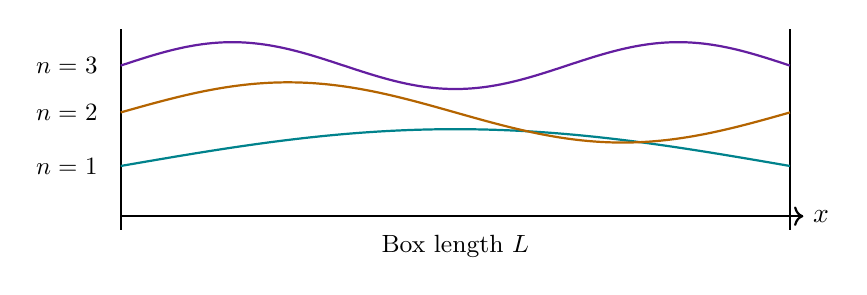
\begin{tikzpicture}[scale=0.85]
  \draw[->, thick] (0,0) -- (10.2,0) node[right] {$x$};
  \draw[thick] (0,-0.2) -- (0,2.8);
  \draw[thick] (10,-0.2) -- (10,2.8);
  \draw[myteal, thick, domain=0:10, samples=100] plot(\x,{0.75+0.55*sin(18*\x)});
  \draw[myamber, thick, domain=0:10, samples=120] plot(\x,{1.55+0.45*sin(36*\x)});
  \draw[mypurple, thick, domain=0:10, samples=140] plot(\x,{2.25+0.35*sin(54*\x)});
  \node[anchor=east, font=\small] at (-0.2,0.75) {$n=1$};
  \node[anchor=east, font=\small] at (-0.2,1.55) {$n=2$};
  \node[anchor=east, font=\small] at (-0.2,2.25) {$n=3$};
  \node[font=\small] at (5,-0.45) {Box length $L$};
\end{tikzpicture}
\end{tcolorbox}

\subsection{Molecular Orbitals of Diatomic Molecules}
Molecular orbital (MO) theory states that atomic orbitals combine to form molecular orbitals spread over the whole molecule. Constructive overlap gives bonding MOs and destructive overlap gives antibonding MOs.

\begin{tcolorbox}[formulabox, title={Bond Order}]
\[
\text{Bond order}=\frac{N_b-N_a}{2}
\]
where $N_b$ is the number of electrons in bonding MOs and $N_a$ is the number of electrons in antibonding MOs. Higher bond order means shorter, stronger bond.
\end{tcolorbox}

\textbf{Important examples:}\par\noindent
\begin{tabularx}{\linewidth}{|B{2.8cm}|Y|Y|Y|}
\hline
\textbf{Molecule} & \textbf{Configuration idea} & \textbf{Bond order} & \textbf{Magnetism} \\
\hline
$\mathrm{H_2}$ & Two electrons in $\sigma_{1s}$ & 1 & Diamagnetic \\
\hline
\hline
\end{tabularx}

\begin{tcolorbox}[tikzbox, title={Molecular Orbital Energy Level Diagram of Oxygen (\texorpdfstring{$\mathrm{O_2}$}{O2})}]
\centering
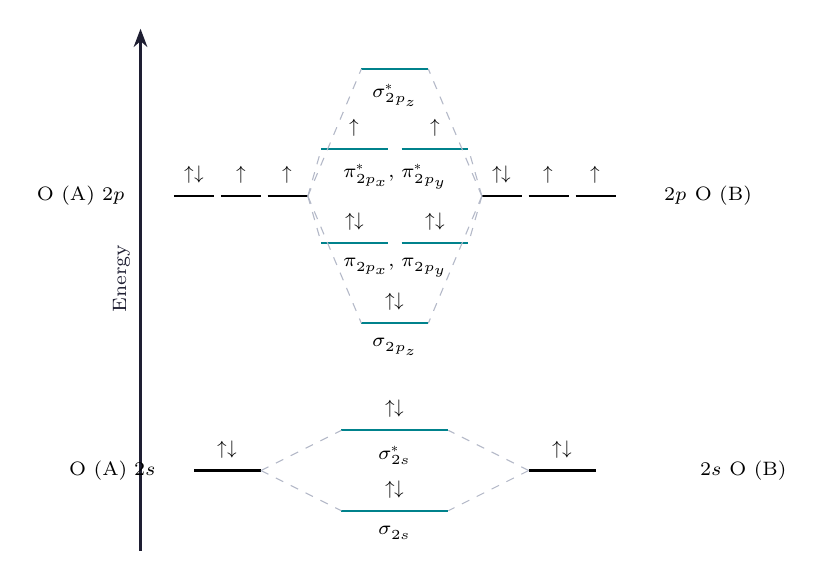
\begin{tikzpicture}[scale=0.85, every node/.style={font=\scriptsize}]
  % Energy axis on the left
  \draw[arrow] (-3.8,-2.6) -- (-3.8,5.2) node[midway, rotate=90, above=4pt] {Energy};

  % --- 2s Orbitals ---
  % AO Left
  \draw[thick] (-3.0,-1.4) -- (-2.0,-1.4) node[left=1.2cm] {O (A) $2s$};
  \node[above=1pt] at (-2.5,-1.4) {$\uparrow\downarrow$};

  % AO Right
  \draw[thick] (2.0,-1.4) -- (3.0,-1.4) node[right=1.2cm] {$2s$ O (B)};
  \node[above=1pt] at (2.5,-1.4) {$\uparrow\downarrow$};

  % MO Center
  \draw[thick, myteal] (-0.8,-2.0) -- (0.8,-2.0);
  \node[below=2pt] at (0,-2.0) {$\sigma_{2s}$};
  \node[above=1pt] at (0,-2.0) {$\uparrow\downarrow$};
  
  \draw[thick, myteal] (-0.8,-0.8) -- (0.8,-0.8);
  \node[below=2pt] at (0,-0.8) {$\sigma^*_{2s}$};
  \node[above=1pt] at (0,-0.8) {$\uparrow\downarrow$};

  % Connecting lines for 2s
  \draw[dashed, mgframe] (-2.0,-1.4) -- (-0.8,-2.0);
  \draw[dashed, mgframe] (-2.0,-1.4) -- (-0.8,-0.8);
  \draw[dashed, mgframe] (2.0,-1.4) -- (0.8,-2.0);
  \draw[dashed, mgframe] (2.0,-1.4) -- (0.8,-0.8);


  % --- 2p Orbitals ---
  % AO Left
  \draw[thick] (-3.3,2.7) -- (-2.7,2.7);
  \draw[thick] (-2.6,2.7) -- (-2.0,2.7);
  \draw[thick] (-1.9,2.7) -- (-1.3,2.7);
  \node[left=2.2cm] at (-1.3,2.7) {O (A) $2p$};
  \node[above=1pt] at (-3.0,2.7) {$\uparrow\downarrow$};
  \node[above=1pt] at (-2.3,2.7) {$\uparrow$};
  \node[above=1pt] at (-1.6,2.7) {$\uparrow$};

  % AO Right
  \draw[thick] (1.3,2.7) -- (1.9,2.7);
  \draw[thick] (2.0,2.7) -- (2.6,2.7);
  \draw[thick] (2.7,2.7) -- (3.3,2.7);
  \node[right=2.2cm] at (1.3,2.7) {$2p$ O (B)};
  \node[above=1pt] at (1.6,2.7) {$\uparrow\downarrow$};
  \node[above=1pt] at (2.3,2.7) {$\uparrow$};
  \node[above=1pt] at (3.0,2.7) {$\uparrow$};

  % MO Center
  \draw[thick, myteal] (-0.5,0.8) -- (0.5,0.8);
  \node[below=2pt] at (0,0.8) {$\sigma_{2p_z}$};
  \node[above=1pt] at (0,0.8) {$\uparrow\downarrow$};

  \draw[thick, myteal] (-1.1,2.0) -- (-0.1,2.0);
  \draw[thick, myteal] (0.1,2.0) -- (1.1,2.0);
  \node[below=2pt] at (0,2.0) {$\pi_{2p_x},\,\pi_{2p_y}$};
  \node[above=1pt] at (-0.6,2.0) {$\uparrow\downarrow$};
  \node[above=1pt] at (0.6,2.0) {$\uparrow\downarrow$};

  \draw[thick, myteal] (-1.1,3.4) -- (-0.1,3.4);
  \draw[thick, myteal] (0.1,3.4) -- (1.1,3.4);
  \node[below=2pt] at (0,3.4) {$\pi^*_{2p_x},\,\pi^*_{2p_y}$};
  \node[above=1pt] at (-0.6,3.4) {$\uparrow$};
  \node[above=1pt] at (0.6,3.4) {$\uparrow$};

  \draw[thick, myteal] (-0.5,4.6) -- (0.5,4.6);
  \node[below=2pt] at (0,4.6) {$\sigma^*_{2p_z}$};

  % Connecting lines for 2p
  \draw[dashed, mgframe] (-1.3,2.7) -- (-0.5,0.8);
  \draw[dashed, mgframe] (-1.3,2.7) -- (-1.1,2.0);
  \draw[dashed, mgframe] (-1.3,2.7) -- (-1.1,3.4);
  \draw[dashed, mgframe] (-1.3,2.7) -- (-0.5,4.6);

  \draw[dashed, mgframe] (1.3,2.7) -- (0.5,0.8);
  \draw[dashed, mgframe] (1.3,2.7) -- (1.1,2.0);
  \draw[dashed, mgframe] (1.3,2.7) -- (1.1,3.4);
  \draw[dashed, mgframe] (1.3,2.7) -- (0.5,4.6);
\end{tikzpicture}
\end{tcolorbox}

\subsection{Pi-Molecular Orbitals and Aromaticity}
Pi-electrons in conjugated systems are delocalized. Benzene has six pi-electrons distributed over six carbon atoms, making it unusually stable.

\begin{tcolorbox}[defbox]
\textbf{Aromatic compound:} A cyclic, planar, fully conjugated molecule having $(4n+2)$ pi-electrons, where $n=0,1,2,\ldots$.
\end{tcolorbox}

\begin{tcolorbox}[tikzbox, title={Benzene Pi-Electron Delocalization}]
\centering
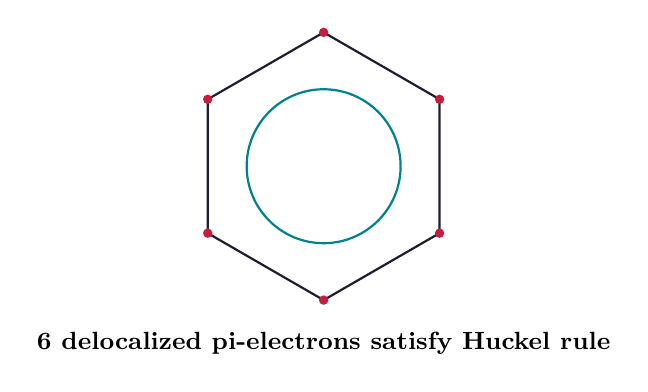
\begin{tikzpicture}[scale=0.85]
  \foreach \i in {1,...,6} {
    \coordinate (C\i) at ({90+60*(\i-1)}:2);
  }
  \draw[thick, color=mydark] (C1)--(C2)--(C3)--(C4)--(C5)--(C6)--cycle;
  \draw[myteal, thick] (0,0) circle (1.15);
  \foreach \i in {1,...,6} \fill[myred] (C\i) circle (2pt);
  \node[font=\small\bfseries] at (0,-2.65) {6 delocalized pi-electrons satisfy Huckel rule};
\end{tikzpicture}
\end{tcolorbox}

\subsection{Pi-Molecular Orbitals of 1,3-Butadiene}
1,3-butadiene ($\mathrm{CH_2=CH-CH=CH_2}$) has a conjugated system of four $p$ orbitals containing four $\pi$ electrons. These combine to form four $\pi$ molecular orbitals ($\psi_1, \psi_2, \psi_3, \psi_4$) with increasing energy and nodes.
\begin{itemize}[leftmargin=*, itemsep=3pt]
  \item \textbf{Nodal Properties:} The number of nodes in orbital $\psi_k$ is equal to $(k-1)$. A node is a position where the wave function changes sign and electron probability is zero.
  \item \textbf{HOMO/LUMO:} In the ground state, the four $\pi$ electrons fill the two lowest-energy orbitals ($\psi_1, \psi_2$). Thus, $\psi_2$ is the \textbf{Highest Occupied Molecular Orbital (HOMO)} and $\psi_3$ is the \textbf{Lowest Unoccupied Molecular Orbital (LUMO)}.
\end{itemize}

\begin{tcolorbox}[tikzbox, title={Pi-Molecular Orbitals of 1,3-Butadiene}]
\centering
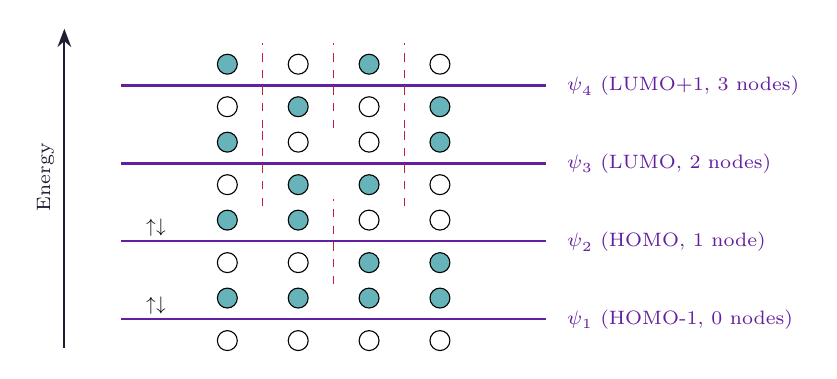
\begin{tikzpicture}[scale=0.9, every node/.style={font=\scriptsize}]
  % Energy axis
  \draw[arrow] (-3.8,-0.5) -- (-3.8,4.0) node[midway, rotate=90, above=4pt] {Energy};

  % --- Level psi_4 (3 nodes) ---
  \draw[thick, mypurple] (-3.0,3.2) -- (3.0,3.2) node[right=4pt] {$\psi_4$ (LUMO+1, 3 nodes)};
  % Draw lobes for + - + -
  \fill[myteal!60] (-1.5,3.5) circle (4pt); \draw (-1.5,3.5) circle (4pt);
  \draw (-1.5,2.9) circle (4pt);
  \draw (-0.5,3.5) circle (4pt);
  \fill[myteal!60] (-0.5,2.9) circle (4pt); \draw (-0.5,2.9) circle (4pt);
  \fill[myteal!60] (0.5,3.5) circle (4pt); \draw (0.5,3.5) circle (4pt);
  \draw (0.5,2.9) circle (4pt);
  \draw (1.5,3.5) circle (4pt);
  \fill[myteal!60] (1.5,2.9) circle (4pt); \draw (1.5,2.9) circle (4pt);
  % Nodes
  \draw[dashed, myred] (-1.0,2.6) -- (-1.0,3.8);
  \draw[dashed, myred] (0.0,2.6) -- (0.0,3.8);
  \draw[dashed, myred] (1.0,2.6) -- (1.0,3.8);

  % --- Level psi_3 (2 nodes) ---
  \draw[thick, mypurple] (-3.0,2.1) -- (3.0,2.1) node[right=4pt] {$\psi_3$ (LUMO, 2 nodes)};
  % Draw lobes for + - - +
  \fill[myteal!60] (-1.5,2.4) circle (4pt); \draw (-1.5,2.4) circle (4pt);
  \draw (-1.5,1.8) circle (4pt);
  \draw (-0.5,2.4) circle (4pt);
  \fill[myteal!60] (-0.5,1.8) circle (4pt); \draw (-0.5,1.8) circle (4pt);
  \draw (0.5,2.4) circle (4pt);
  \fill[myteal!60] (0.5,1.8) circle (4pt); \draw (0.5,1.8) circle (4pt);
  \fill[myteal!60] (1.5,2.4) circle (4pt); \draw (1.5,2.4) circle (4pt);
  \draw (1.5,1.8) circle (4pt);
  % Nodes
  \draw[dashed, myred] (-1.0,1.5) -- (-1.0,2.7);
  \draw[dashed, myred] (1.0,1.5) -- (1.0,2.7);

  % --- Level psi_2 (1 node) ---
  \draw[thick, mypurple] (-3.0,1.0) -- (3.0,1.0) node[right=4pt] {$\psi_2$ (HOMO, 1 node)};
  \node at (-2.5, 1.2) {$\uparrow\downarrow$};
  % Draw lobes for + + - -
  \fill[myteal!60] (-1.5,1.3) circle (4pt); \draw (-1.5,1.3) circle (4pt);
  \draw (-1.5,0.7) circle (4pt);
  \fill[myteal!60] (-0.5,1.3) circle (4pt); \draw (-0.5,1.3) circle (4pt);
  \draw (-0.5,0.7) circle (4pt);
  \draw (0.5,1.3) circle (4pt);
  \fill[myteal!60] (0.5,0.7) circle (4pt); \draw (0.5,0.7) circle (4pt);
  \draw (1.5,1.3) circle (4pt);
  \fill[myteal!60] (1.5,0.7) circle (4pt); \draw (1.5,0.7) circle (4pt);
  % Nodes
  \draw[dashed, myred] (0.0,0.4) -- (0.0,1.6);

  % --- Level psi_1 (0 nodes) ---
  \draw[thick, mypurple] (-3.0,-0.1) -- (3.0,-0.1) node[right=4pt] {$\psi_1$ (HOMO-1, 0 nodes)};
  \node at (-2.5, 0.1) {$\uparrow\downarrow$};
  % Draw lobes for + + + +
  \fill[myteal!60] (-1.5,0.2) circle (4pt); \draw (-1.5,0.2) circle (4pt);
  \draw (-1.5,-0.4) circle (4pt);
  \fill[myteal!60] (-0.5,0.2) circle (4pt); \draw (-0.5,0.2) circle (4pt);
  \draw (-0.5,-0.4) circle (4pt);
  \fill[myteal!60] (0.5,0.2) circle (4pt); \draw (0.5,0.2) circle (4pt);
  \draw (0.5,-0.4) circle (4pt);
  \fill[myteal!60] (1.5,0.2) circle (4pt); \draw (1.5,0.2) circle (4pt);
  \draw (1.5,-0.4) circle (4pt);
\end{tikzpicture}
\end{tcolorbox}

\subsection{Crystal Field Theory}
In transition-metal complexes, surrounding ligands split the five degenerate $d$ orbitals into different energy groups. The splitting controls colour, magnetic behaviour, and stability.

\begin{tcolorbox}[tikzbox, title={Octahedral Crystal Field Splitting}]
\centering
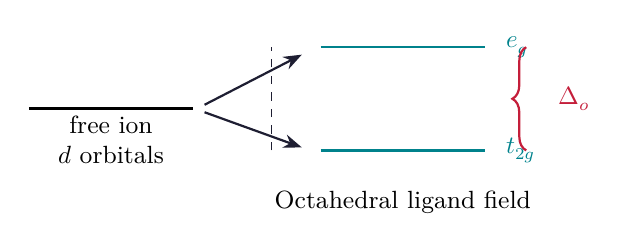
\begin{tikzpicture}[scale=0.95]
  \draw[thick] (0,0) -- (2.2,0);
  \node[font=\small, align=center] at (1.1,-0.42) {free ion\\$d$ orbitals};

  \draw[arrow] (2.35,0.05) -- (3.65,0.72);
  \draw[arrow] (2.35,-0.05) -- (3.65,-0.52);

  \draw[thick,myteal] (3.9,0.82) -- (6.1,0.82);
  \node[font=\small\bfseries\color{myteal}, anchor=west] at (6.25,0.82) {$e_g$};

  \draw[thick,myteal] (3.9,-0.56) -- (6.1,-0.56);
  \node[font=\small\bfseries\color{myteal}, anchor=west] at (6.25,-0.56) {$t_{2g}$};

  \draw[dashed,mydark] (3.25,-0.56) -- (3.25,0.82);
  \draw[decorate, decoration={brace, amplitude=5pt}, thick, myred] (6.65,-0.56) -- (6.65,0.82)
    node[midway,right=8pt,font=\small\bfseries\color{myred}] {$\Delta_o$};
  \node[font=\small] at (5.0,-1.25) {Octahedral ligand field};
\end{tikzpicture}
\end{tcolorbox}

\subsection{Band Structure and Doping}
In solids, many atomic orbitals combine to form bands. Conductivity depends on the band gap $E_g$ between valence band and conduction band.

\begin{tabularx}{\linewidth}{|B{3cm}|Y|Y|}
\hline
\textbf{Material} & \textbf{Band gap} & \textbf{Electrical behaviour} \\
\hline
Conductor & Overlapping bands or very small gap & Electrons move easily \\
\hline
Semiconductor & Moderate gap, about $1$--$3\ \mathrm{eV}$ & Conductivity increases by heat or doping \\
\hline
Insulator & Large gap, usually $>5\ \mathrm{eV}$ & Very poor conductor \\
\hline
\end{tabularx}

\begin{tcolorbox}[exambox, title={Exam Points}]
\begin{itemize}[leftmargin=*, itemsep=2pt, topsep=2pt]
  \item Derive $E_n=n^2h^2/(8mL^2)$ using boundary conditions.
  \item For MO questions, always calculate bond order and then state magnetic nature.
  \item For CFT, mention splitting pattern, $\Delta_o$, high spin or low spin, and magnetic moment.
  \item For band theory, draw valence band, conduction band, and band gap.
\end{itemize}
\end{tcolorbox}

% ===============================================================================
\section{Exam-Oriented Derivations and Applications}
% ===============================================================================

\subsection{Derivation of Particle in a Box Energy}
For a one-dimensional box, potential energy inside the box is zero. Therefore the Schrodinger equation becomes:
\[
-\frac{h^2}{8\pi^2m}\frac{d^2\psi}{dx^2}=E\psi
\]
Rearranging,
\[
\frac{d^2\psi}{dx^2}+\frac{8\pi^2mE}{h^2}\psi=0
\]
Let
\[
k^2=\frac{8\pi^2mE}{h^2}
\]
Then the differential equation becomes:
\[
\frac{d^2\psi}{dx^2}+k^2\psi=0
\]
Its general solution is:
\[
\psi=A\sin kx+B\cos kx
\]
Boundary condition at $x=0$ gives $B=0$. Boundary condition at $x=L$ gives:
\[
A\sin kL=0
\]
For a non-zero wave function:
\[
kL=n\pi,\qquad k=\frac{n\pi}{L}
\]
Substituting in $k^2=8\pi^2mE/h^2$:
\[
E_n=\frac{n^2h^2}{8mL^2}
\]

\begin{tcolorbox}[examplebox, title={Solved Example: Energy Level Ratio}]
\textbf{Problem:} Find the ratio of the first three energy levels for a particle in a box.

\textbf{Solution:} Since $E_n\propto n^2$,
\[
E_1:E_2:E_3=1^2:2^2:3^2=1:4:9
\]
\textbf{Exam note:} Energy gaps are not equal; they increase with $n$.
\end{tcolorbox}

\subsection{MO Filling Order and Magnetic Behaviour}
For second-period diatomic molecules, MO ordering changes after $\mathrm{N_2}$ because $s$-$p$ mixing becomes less important. This is a common exam trap.

\begin{tabularx}{\linewidth}{|B{3.5cm}|Y|Y|}
\hline
\textbf{Molecules} & \textbf{MO order to remember} & \textbf{Important result} \\
\hline
$\mathrm{B_2,C_2,N_2}$ & $\sigma_{2s}<\sigma^*_{2s}<\pi_{2p}<\sigma_{2p}<\pi^*_{2p}<\sigma^*_{2p}$ & $\mathrm{B_2}$ is paramagnetic; $\mathrm{N_2}$ has bond order 3 \\
\hline
$\mathrm{O_2,F_2,Ne_2}$ & $\sigma_{2s}<\sigma^*_{2s}<\sigma_{2p}<\pi_{2p}<\pi^*_{2p}<\sigma^*_{2p}$ & $\mathrm{O_2}$ is paramagnetic due to two unpaired electrons \\
\hline
\end{tabularx}

\begin{tcolorbox}[examplebox, title={Solved Example: Bond Order of Oxygen}]
For $\mathrm{O_2}$, total valence electrons are $12$.
\[
N_b=8,\qquad N_a=4
\]
\[
\text{Bond order}=\frac{8-4}{2}=2
\]
Two electrons remain unpaired in $\pi^*_{2p}$ orbitals, so oxygen is \textbf{paramagnetic}.
\end{tcolorbox}

\subsection{Crystal Field Splitting: High Spin and Low Spin}
In octahedral complexes, electrons first occupy lower $t_{2g}$ orbitals. Whether pairing occurs depends on the relative values of crystal field splitting energy $\Delta_o$ and pairing energy $P$.

\begin{tabularx}{\linewidth}{|B{3.2cm}|Y|Y|}
\hline
\textbf{Case} & \textbf{Condition} & \textbf{Result} \\
\hline
High spin complex & $\Delta_o<P$ & Electrons avoid pairing; more unpaired electrons; usually weak-field ligands \\
\hline
Low spin complex & $\Delta_o>P$ & Electrons pair in $t_{2g}$ before occupying $e_g$; fewer unpaired electrons; usually strong-field ligands \\
\hline
\end{tabularx}

\begin{tcolorbox}[tikzbox, title={High Spin and Low Spin Choice for Octahedral Complexes}]
\centering
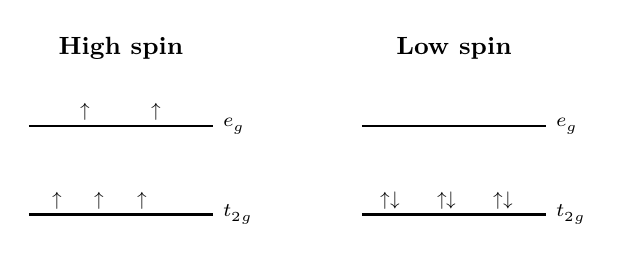
\begin{tikzpicture}[scale=0.9]
  \node[font=\small\bfseries] at (1.3,2.35) {High spin};
  \draw[thick] (0,0) -- (2.6,0) node[right,font=\scriptsize] {$t_{2g}$};
  \draw[thick] (0,1.25) -- (2.6,1.25) node[right,font=\scriptsize] {$e_g$};
  \foreach \x in {0.4,1.0,1.6} \node[font=\scriptsize] at (\x,0.2) {$\uparrow$};
  \foreach \x in {0.8,1.8} \node[font=\scriptsize] at (\x,1.45) {$\uparrow$};

  \node[font=\small\bfseries] at (6.0,2.35) {Low spin};
  \draw[thick] (4.7,0) -- (7.3,0) node[right,font=\scriptsize] {$t_{2g}$};
  \draw[thick] (4.7,1.25) -- (7.3,1.25) node[right,font=\scriptsize] {$e_g$};
  \foreach \x in {5.1,5.9,6.7} \node[font=\scriptsize] at (\x,0.2) {$\uparrow\downarrow$};
\end{tikzpicture}
\end{tcolorbox}

\subsection{n-Type and p-Type Semiconductors}
Doping adds controlled impurities to a semiconductor. Pentavalent dopants such as P or As introduce donor levels and produce n-type semiconductors. Trivalent dopants such as B or Al introduce acceptor levels and produce p-type semiconductors.

\begin{tcolorbox}[tikzbox, title={Doping Levels in Semiconductors}]
\centering
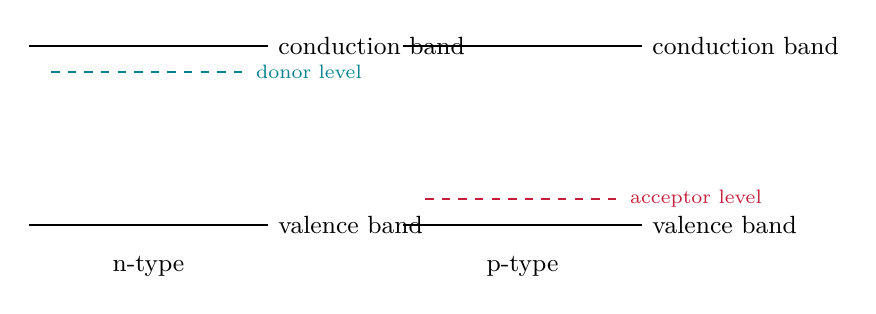
\begin{tikzpicture}[scale=0.95]
  \draw[thick] (0,0) -- (3.2,0) node[right,font=\small] {valence band};
  \draw[thick] (0,2.4) -- (3.2,2.4) node[right,font=\small] {conduction band};
  \draw[myteal, thick, dashed] (0.3,2.05) -- (2.9,2.05) node[right,font=\scriptsize] {donor level};
  \node[font=\small] at (1.6,-0.55) {n-type};

  \draw[thick] (5,0) -- (8.2,0) node[right,font=\small] {valence band};
  \draw[thick] (5,2.4) -- (8.2,2.4) node[right,font=\small] {conduction band};
  \draw[myred, thick, dashed] (5.3,0.35) -- (7.9,0.35) node[right,font=\scriptsize] {acceptor level};
  \node[font=\small] at (6.6,-0.55) {p-type};
\end{tikzpicture}
\end{tcolorbox}

\begin{tcolorbox}[masonbox, title={How to Write 10-Mark Answers in This Module}]
\begin{enumerate}[leftmargin=*, itemsep=3pt, topsep=2pt]
  \item Start with a definition in 2--3 lines.
  \item Draw the required energy-level or orbital diagram.
  \item Write the governing formula with symbol meanings.
  \item Add one example such as $\mathrm{O_2}$ paramagnetism, benzene aromaticity, or n-type doping.
  \item End with one application or exam conclusion.
\end{enumerate}
\end{tcolorbox}

\subsection{Important Long-Answer: Aromaticity of Benzene}
Benzene is the standard example of aromatic stability. A complete answer should not only state Huckel rule, but also connect structure, pi-electron count, planarity, and equal bond lengths.

\begin{enumerate}[leftmargin=*, itemsep=3pt, topsep=2pt]
  \item Benzene is cyclic and planar, so all six carbon atoms can overlap through unhybridized $p$ orbitals.
  \item Each carbon contributes one pi-electron, giving a total of six pi-electrons.
  \item Huckel rule requires $(4n+2)$ pi-electrons. For benzene:
  \[
    4n+2=6\quad\Rightarrow\quad n=1
  \]
  \item The pi-electrons are delocalized above and below the ring.
  \item Delocalization makes all C--C bonds equivalent and gives extra stability.
\end{enumerate}

\begin{tcolorbox}[examplebox, title={Exam Comparison: Aromatic, Anti-Aromatic and Non-Aromatic}]
\begin{tabularx}{\linewidth}{|B{3.0cm}|Y|Y|Y|}
\hline
\textbf{Type} & \textbf{Condition} & \textbf{Pi-electrons} & \textbf{Example idea} \\
\hline
Aromatic & Cyclic, planar, conjugated & $(4n+2)$ & Benzene, cyclopentadienyl anion \\
\hline
Anti-aromatic & Cyclic, planar, conjugated & $4n$ & Cyclobutadiene type systems \\
\hline
Non-aromatic & Fails planarity or conjugation & Rule not applicable & Non-planar or saturated ring \\
\hline
\end{tabularx}
\end{tcolorbox}

\subsection{Important Long-Answer: Crystal Field Theory and Magnetism}
Crystal field theory explains colour and magnetic properties of transition metal complexes by ligand-induced splitting of $d$ orbitals.

\begin{tcolorbox}[formulabox, title={Crystal Field Stabilization Energy}]
For an octahedral complex:
\[
\mathrm{CFSE}=(-0.4x+0.6y)\Delta_o+pP
\]
where $x$ is the number of electrons in $t_{2g}$ orbitals, $y$ is the number of electrons in $e_g$ orbitals, and $pP$ is the pairing energy contribution.
\end{tcolorbox}

\begin{tcolorbox}[examplebox, title={Solved Example: Octahedral \texorpdfstring{$d^3$}{d3} Configuration}]
For a $d^3$ octahedral ion, electrons occupy $t_{2g}$ orbitals singly:
\[
t_{2g}^3e_g^0
\]
\[
\mathrm{CFSE}=3(-0.4\Delta_o)=-1.2\Delta_o
\]
There are three unpaired electrons, so the spin-only magnetic moment is:
\[
\mu=\sqrt{3(3+2)}=\sqrt{15}=3.87\ \mathrm{BM}
\]
\end{tcolorbox}

\subsection{Band Theory: Exam Numericals and Concepts}
Band gap decides electrical behaviour. If the gap is small, thermal energy can excite electrons to the conduction band. Doping reduces the effective energy needed for charge conduction.

\begin{tabularx}{\linewidth}{|B{3.2cm}|Y|Y|}
\hline
\textbf{Question type} & \textbf{What to write} & \textbf{Common conclusion} \\
\hline
Conductor vs semiconductor & Draw overlapping band and small band gap & Conductor has many free electrons \\
\hline
Intrinsic semiconductor & Pure semiconductor with thermally generated carriers & Electron and hole concentrations are equal \\
\hline
n-type semiconductor & Donor level near conduction band & Electrons are majority carriers \\
\hline
p-type semiconductor & Acceptor level near valence band & Holes are majority carriers \\
\hline
\end{tabularx}

\begin{tcolorbox}[masonbox, title={Previous-Year Style Questions}]
\begin{enumerate}[leftmargin=*, itemsep=4pt, topsep=2pt]
  \item Derive the energy expression for a particle in a one-dimensional box and explain why $n=0$ is not allowed.
  \item Draw the MO diagram of $\mathrm{O_2}$ and explain its paramagnetic nature.
  \item Explain aromaticity of benzene using Huckel rule.
  \item Explain high-spin and low-spin octahedral complexes with suitable examples.
  \item Compare conductors, semiconductors and insulators using band theory.
\end{enumerate}
\end{tcolorbox}
\newpage
\begin{center}
  {\large\bfseries\color{myred} Quick Revision --- Module 1}\\[3pt]
  {\small\color{mydark} Atomic and Molecular Structure $|$ BS-CH101}
\end{center}
\noindent{\color{myred}\rule{\linewidth}{1.2pt}}
\vspace{4pt}

\begin{tcolorbox}[formulabox, title={Key Formulas at a Glance}]
\begin{tabularx}{\linewidth}{|B{4.0cm}|Y|}
\hline
\textbf{Formula / Rule} & \textbf{Meaning} \\
\hline
$\hat{H}\psi=E\psi$ & Schrodinger eigenvalue equation for allowed energies. \\
\hline
$E_n=\displaystyle\frac{n^2h^2}{8mL^2}$ & Energy of a particle in a one-dimensional box. \\
\hline
$\psi_n=\sqrt{\displaystyle\frac{2}{L}}\sin\displaystyle\frac{n\pi x}{L}$ & Normalized wave function for a particle in a box. \\
\hline
$\text{Bond order}=\displaystyle\frac{N_b-N_a}{2}$ & Predicts bond strength and stability in MO theory. \\
\hline
$\mu=\sqrt{n(n+2)}\ \mathrm{BM}$ & Spin-only magnetic moment for $n$ unpaired electrons. \\
\hline
$4n+2$ & Huckel rule for aromatic pi-electron count. \\
\hline
\end{tabularx}
\end{tcolorbox}

\begin{tcolorbox}[defbox, title={One-Line Definitions}]
\begin{itemize}[leftmargin=*, itemsep=2pt, topsep=2pt]
  \item \textbf{Wave function:} Mathematical function whose square gives probability density.
  \item \textbf{Node:} Point or surface where $\psi=0$.
  \item \textbf{Bonding MO:} Lower-energy MO formed by constructive overlap.
  \item \textbf{Antibonding MO:} Higher-energy MO formed by destructive overlap.
  \item \textbf{Aromaticity:} Extra stability due to cyclic delocalization of $(4n+2)$ pi-electrons.
  \item \textbf{Crystal field splitting:} Separation of metal $d$ orbitals in a ligand field.
  \item \textbf{Band gap:} Energy gap between valence and conduction bands.
\end{itemize}
\end{tcolorbox}

\begin{tcolorbox}[exambox, title={Frequently Asked / Viva Questions}]
\begin{enumerate}[topsep=0pt, label=\textbf{Q\arabic*.}, itemsep=5pt]
  \item \Q{State the Schrodinger equation.}
    The time-independent form is $\hat{H}\psi=E\psi$, where $\hat{H}$ is the energy operator.
  \item \Q{Why is energy quantized for a particle in a box?}
    Only wave functions satisfying $\psi(0)=0$ and $\psi(L)=0$ are allowed, giving discrete $n$ values.
  \item \Q{What is the zero-point energy?}
    The minimum energy of a confined particle, $E_1=h^2/(8mL^2)$.
  \item \Q{Define bond order.}
    Bond order is $(N_b-N_a)/2$; it measures net bonding in a molecule.
  \item \Q{Why is oxygen paramagnetic?}
    $\mathrm{O_2}$ has two unpaired electrons in antibonding $\pi^*$ orbitals.
  \item \Q{What is Huckel rule?}
    A cyclic planar conjugated molecule is aromatic if it has $(4n+2)$ pi-electrons.
  \item \Q{Why is benzene stable?}
    Six pi-electrons are delocalized over the ring, satisfying Huckel rule with $n=1$.
  \item \Q{What is crystal field splitting?}
    Splitting of metal $d$ orbitals into groups of different energy by ligands.
  \item \Q{What is the role of doping in semiconductors?}
    Doping introduces donor or acceptor levels and increases carrier concentration.
  \item \Q{How are conductors and insulators distinguished by band theory?}
    Conductors have overlapping or nearly touching bands, whereas insulators have a large band gap.
\end{enumerate}
\end{tcolorbox}

\begin{tcolorbox}[tikzbox, title={Summary Reference Table}]
\begin{tabularx}{\linewidth}{|B{3.2cm}|Y|Y|}
\hline
\textbf{Topic} & \textbf{Key idea} & \textbf{Exam output} \\
\hline
Particle in box & Boundary conditions give discrete energies & Derivation plus energy-level diagram \\
\hline
MO theory & Atomic orbitals combine into bonding and antibonding MOs & Bond order and magnetism \\
\hline
CFT & Ligands split $d$ orbitals & Splitting diagram and unpaired electrons \\
\hline
Band theory & Bands decide electrical conductivity & Conductor, semiconductor, insulator comparison \\
\hline
\end{tabularx}
\end{tcolorbox}

\end{document}
